この章では, 2章で説明したEdDSAの性能と5章で示した実験結果から, 
EdDSAの実装評価をする. はじめに, 5章で示した実験結果の評価を
他の認証方式と比較しながらまとめ, その後に2章の内容を含めながら
ECDSAとの総合的な比較評価を行う. 最後に, 本研究で行った実験結果から
想定されるEdDSAの利用シーンについて考察する.\\[1em]
\noindent {\large\textbf{実験結果のまとめ}} 
\begin{enumerate}
  \item 実験1\\
  \indent EdDSAを用いたことで, 不正ノードを排除することができたが, 
  他の認証方式との差は見られなかった. 
  \item 実験2\\
  \indent 平均遅延と平均パケット配送率において, EdDSAは他の
  認証方式との差は見られなかったが, それぞれの鍵長の違いから
  オーバーヘッドサイズがDSAよりも小さく, ECDSAと同程度であった.
  \item 実験3\\
  \indent EdDSAは他の認証方式よりも署名の生成と検証にかかる時間が
  短いことから, 処理能力(計算効率)が高いことがわかった.
\end{enumerate}

\noindent {\large\textbf{EdDSAとECDSAの比較評価}}\\
\indent 上記の実験結果のまとめから, EdDSAはECDSAよりも
計算効率が高いことがわかった. これは, 第2章で述べたEdDSAの設計上の
特長である高速な処理能力が実験環境においても十分に発揮されたことを
示している. また, 第2章で述べたセキュリティの堅牢性から, 
EdDSAは秘密鍵を特定しようとする攻撃者が存在する環境でECDSAよりも
高いセキュリティを提供できる. よって, V2Vアドホックネットワーク
において, EdDSAはECDSAよりも安全かつ効率的な認証方式として
利用できるといえる.\\

\noindent {\large\textbf{EdDSAの利用シーンについての考察}}\\
\indent シミュレーション実験からEdDSAは他の認証方式, 特にECDSAと比べても
通信品質が向上, または同等であることがわかった. さらに, 実験2で採取したデータに
メモリ使用量がある. 図\ref{fig:memory_usages}に示すように,   
Ed25519のメモリの使用量がECDSAよりも少ないことがわかる. 
また, 本研究の実験環境では, EdDSAの署名の生成と検証の時間が
データパケットとHelloパケットの送信間隔(1秒)に比べて非常に短いということから, 
次のような環境であれば署名の生成と検証の回数がより多くなり, 
EdDSAの処理効率を最大限に発揮できると考えられる. 
\begin{itemize}
  \item ノード数が非常に多い
  \item データパケットとHelloパケットの送信間隔が非常に短い
  \item 使えるリソースが限られている
\end{itemize}
さらに, 次のような環境であればEdDSAのセキュリティの堅牢さを
発揮すると考えられる. 
\begin{itemize}
  \item 秘密鍵を特定しようとする攻撃者が存在する
\end{itemize} 
% \par\indent 以上のことから, EdDSAはV2VアドホックネットワークやIoT
% が発展していく中で, 今後ますます重要な役割を果たすと考えられる.\\

\begin{figure}
  \centering
  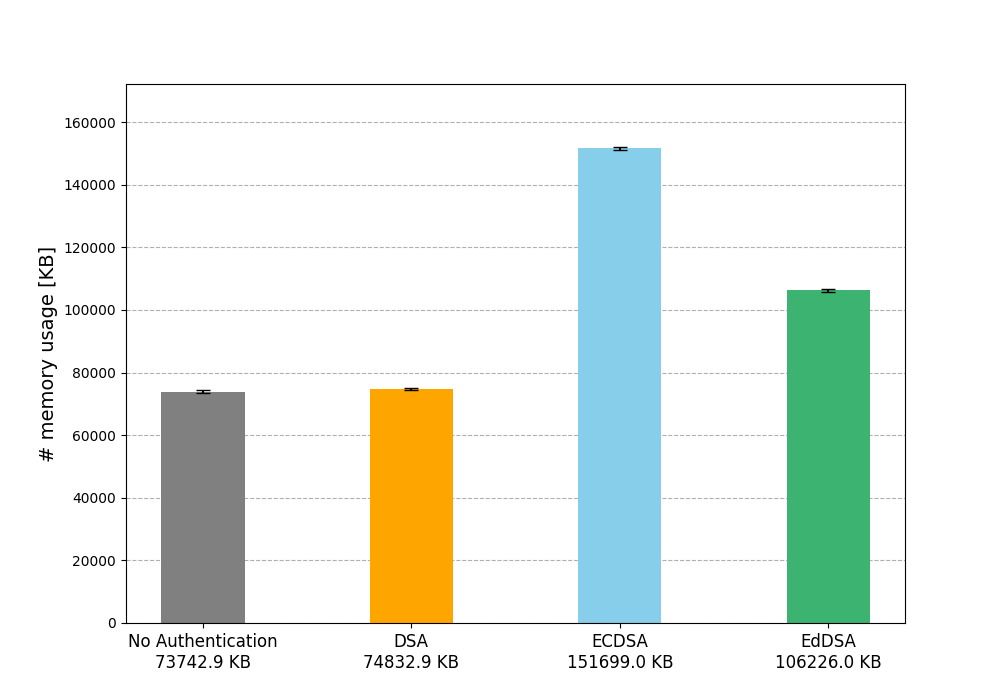
\includegraphics[width=1\textwidth]{figures/memory_usages.png}
  \caption{メモリ使用量}
  \label{fig:memory_usages}
\end{figure}






